%====================================
% build with arara:
%====================================
%
%
%
% !TEX TS-program = arara
% arara: clean: {files: [thesis_main.bbl, thesis_main.aux, thesis_main.pdf]}
% arara: xelatex
% arara: nomencl
% arara: biber
% arara: xelatex
% arara: xelatex
% arara: clean: {files: [thesis_main.out, thesis_main.toc, thesis_main.lot, thesis_main.lof, thesis_main.bbl, thesis_main.nls, thesis_main.nlo, thesis_main.aux, thesis_main.idx, thesis_main.ilg, thesis_main.ind, thesis_main.bbl, thesis_main.bcf, thesis_main.ist, thesis_main.blg, thesis_main.run.xml]}
%
%
%
%====================================
% compile with XeLaTeX
% LuaLaTeX not tested
% pdflatex won't compile
%          for good reason
%====================================
% Präambel
%====================================
% Definition des Dokuments
% inkl. Kopfzeile
%====================================
\documentclass[12pt,oneside,titlepage,listof=totoc,bibliography=totoc]{scrartcl}
\usepackage[
	a4paper,
	top=4cm,
	bottom=2cm,
	left=4cm,
	right=2cm,
	headheight=2cm, %head height
	footskip=2cm, %Abstand footer zu Text
	headheight=2cm,
	heightrounded, %Runden der Höhe
]{geometry} %https://mirror.hmc.edu/ctan/macros/latex/contrib/geometry-de/geometry-de.pdf
%====================================
% Pakete
%====================================
\usepackage{thesis_main_style}
%====================================
% Sprachsupport Pakete
%====================================
%\usepackage{polyglossia} %required for compiling - http://ctan.math.illinois.edu/macros/latex/contrib/polyglossia/polyglossia.pdf
%\setdefaultlanguage[spelling=new]{german} %required for compiling, muiltilanguage support possible - https://latexkurs.github.io/lecture/08_bibliografien_mehrsprachigkeit.pdf
%\usepackage[german=quotes]{csquotes} %required for compiling
%====================================
% Skriptdateien Einbinden
%====================================
\addbibresource{Deine_Inhalte/Literatur/Literatur.bib} %Bib-Datei einbinden
\graphicspath{{./}{./Deine_Inhalte/}{./Deine_Inhalte/Abbildungen/}{./Deine_Inhalte/Kapitel}} % Pfad fuer Abbildungen %{{./}{./abbildungen/}}
\usepackage{titletoc}

\makeatletter

% Setze die Tiefe des Inhaltsverzeichnis auf 4 Ebenen%
% Damit erscheinen \paragraph-Sektionen auch im Inhaltsverzeichnis
\setcounter{secnumdepth}{4}
\setcounter{tocdepth}{4}

% Fuege Abstand nach unten wie in einer normalen \section hinzu
% Andernfalls haette \paragraph keinen Zeilenumbruch
% Der Zeilenumbruch koennte mit einer leeren \mbox{} ersetzt werden
% Jedoch klebt dann der Text relativ nah an der Ueberschrift
\renewcommand{\paragraph}{%
  \@startsection{paragraph}{4}%
  {\z@}{3.25ex \@plus 1ex \@minus .2ex}{1.5ex plus 0.2ex}%
  {\normalfont\normalsize\bfseries\rmfamily}%
}
% TODO Abstand über Titel
\makeatother
 % Weitere Ebene einfügen
%====================================
% Abkürzungsverzeichnis
%====================================
\usepackage[intoc]{nomencl}
\renewcommand{\nomname}{Abkürzungsverzeichnis}
\setlength{\nomlabelwidth}{.50\textwidth}
\renewcommand{\nomlabel}[1]{#1 \dotfill}
\setlength{\nomitemsep}{-\parsep}
\makenomenclature
%========================================================================
% Meta Informationen
% Hier gibts du deine Daten ein!!!
%========================================================================
%-----------------------------------
% Meta Informationen:
% zu dir und deiner Arbeit!!!
%-----------------------------------

% Autor_1
\newcommand{\myAutorEins}{Florentina Fommie}
% Adresse_1
\newcommand{\myAdresseEins}{Platzl 11}
% Stadt_1
\newcommand{\myStadtEins}{80331 München}

% Autor_2
%\newcommand{\myAutorZwei}{Max Mustermann}
% Adresse_2
%\newcommand{\myAdresseZwei}{Musterstr. 24}
% Stadt_2
%\newcommand{\myStadtZwei}{80331 München}

% Titel der Arbeit
\newcommand{\myTitel}{Eine FOM-\LaTeX{}-Vorlage mit \XeLaTeX-Engine, Biblatex und arara Buildtool}

% Betreuer
\newcommand{\myBetreuer}{Professor X. Xaviar}

% Lehrveranstaltung
\newcommand{\myLehrveranstaltung}{Wirtschaftsinformatik Basics 2019 WS}

% Matrikelnummer_1
\newcommand{\myMatrikelNrEins}{914431}
% Matrikelnummer_2
%\newcommand{\myMatrikelNrZwei}{971132}
% Matrikelnummer_3
%\newcommand{\myMatrikelNrDrei}{923456}

% Ort
\newcommand{\myOrt}{München}

% Datum der Abgabe
\newcommand{\myAbgabeDatum}{28. Februar 2019}

% Semesterzahl
\newcommand{\mySemesterZahl}{7}

% Name der Hochschule
\newcommand{\myHochschulName}{FOM Hochschule für Oekonomie \& Management}

% Standort der Hochschule
\newcommand{\myHochschulStandort}{Studienzentrum München}

% Studiengang
\newcommand{\myStudiengang}{Wirtschaftsinformatik}

% Art der Arbeit
\newcommand{\myThesisArt}{Hausarbeit}
%\newcommand{\myThesisArt}{Bachelor Thesis}

% Zu erlangender akademische Grad
\newcommand{\myAkademischerGrad}{Bachelor of Science \(B. Sc.\)}

% Firma
\newcommand{\myFirma}{Mustermann GmbH}
%====================================
% Kopfzeile / Header definieren
% Fußzeile / Footer definieren
% Seitenzahlen definieren
%====================================
\fancypagestyle{plain}{%
	\fancyhf{} %clear header and footer fields
	\fancyhead[C]{\thepage}
	\fancyfoot{}
	\renewcommand{\headrulewidth}{0pt}
	\renewcommand{\footrulewidth}{0pt}
} %redefine plain style
\pagestyle{fancy} %define site style
	\fancyhf{} %clear header and footer fields
	\fancyhead[C]{\thepage}
	\fancyfoot{}
	%\chead{\thepage}
	\renewcommand{\headrulewidth}{0pt}
	\renewcommand{\footrulewidth}{0pt}
%====================================
% Ab hier startet dein Dokument!!!
%====================================
\begin{document}
	\renewcommand{\figurename}{Abbildung} 			%Bildunterschrift
	\pagenumbering{Roman}							% Seitennumerierung auf römisch umstellen
\renewcommand{\refname}{Literaturverzeichnis}		% "Literaturverzeichnis" benennen
\newcolumntype{C}{>{\centering\arraybackslash}X}	% Neuer Tabellen-Spalten-Typ: Zentriert und umbrechbar
%========================================================================
% Titlelseite Stand: Dezember 2016
%========================================================================
 \begin{titlepage}
    \newgeometry{left=2cm, right=2cm, top=.5cm, bottom=2cm}
    \begin{center}
        \vspace{.5cm}
        
\includegraphics[width=3cm]{fomLogo} \\
        \vspace{.5cm}
        \textbf{\LARGE \myHochschulName}\\
        \vspace{.5cm}
        \textmd{\Large \myHochschulStandort}\\
        \vspace{.5cm}
        \textmd{\normalsize Berufsbegleitender Studiengang}\\
        \textmd{\normalsize \myStudiengang, \mySemesterZahl. Semester}\\
        \vspace{2cm}
        \textbf{\LARGE \myThesisArt}\\
        \vspace{2cm}
        %==========================================================
        % Text für die Bachelorarbeit aktivieren
        %==========================================================
        %\textmd{zur Erlangung des Grades eines}\\
        %\textmd{\myAkademischerGrad}\\
        %==========================================================
        \textmd{\normalsize im Rahmen der Lehrveranstaltung}\\
        \vspace{.5cm}
        \textmd{\Large \myLehrveranstaltung}\\
        \vspace{2cm}
        \textmd{\normalsize über das Thema}\\
        \vspace{.5cm}
        \textbf{\LARGE \myTitel}\\
        \vspace{0.2cm}
    \end{center}
    \normalsize
    \vfill
    \begin{tabular*}{0.50\textwidth}{@{\extracolsep{\fill}}p{4cm}l}
        Betreuender Dozent: & \myBetreuer \\
        \ &
        \\
        Autoren: & \myAutorEins
        \\
        Matrikelnummer: & \myMatrikelNrEins
        \\
        Adresse: & \myAdresseEins
        \\
        \ & \myStadtEins
        \\
        Abgabe: & \myAbgabeDatum
        \\
    \end{tabular*}
\end{titlepage}



\begin{comment}
TITELSEITE FÜR ZWEI AUHOREN
\begin{titlepage}
    \newgeometry{left=2cm, right=2cm, top=.5cm, bottom=2cm}
    \begin{center}
        \vspace{.5cm}
        
\includegraphics[width=3cm]{Deine_Inhalte/Abbildungen/fomLogo.jpg} \\
        \vspace{.5cm}
        \textbf{\LARGE \myHochschulName}\\
        \vspace{.5cm}
        \textmd{\Large \myHochschulStandort}\\
        \vspace{.5cm}
        \textmd{\normalsize Berufsbegleitender Studiengang}\\
        \textmd{\normalsize \myStudiengang, \mySemesterZahl. Semester}\\
        \vspace{2cm}
        \textbf{\LARGE \myThesisArt}\\
        \vspace{2cm}
        %\textmd{zur Erlangung des Grades eines}\\
        %\textmd{\myAkademischerGrad}\\
        % Oder für Hausarbeiten:
        \textmd{\normalsize im Rahmen der Lehrveranstaltung}\\
        \vspace{.5cm}
        \textmd{\Large \myLehrveranstaltung}\\
        \vspace{2cm}
        \textmd{\normalsize über das Thema}\\
        \vspace{.5cm}
        \textbf{\LARGE \myTitel}\\
        \vspace{0.2cm}
    \end{center}
    \normalsize
    \vfill
    \begin{tabular*}{0.90\textwidth}{@{\extracolsep{\fill}}lll}
        %\begin{tabular*}{0.90\textwidth}{@{\extracolsep{\fill}}|l|l|l|}
        %\hline
        Betreuender Dozent: & \multicolumn{2}{l}{\myBetreuer} \\ % ggf. multicolmn erweitern bei mehreren Autoren
        %\hline
        \ & \ & \\
        %\hline
        Autoren: & \myAutorEins & \myAutorZwei\\
        %\hline
        %Autoren: & \myAutorEins & \myAutorZwei & \myAutorDrei\\
        Matrikelnr.: & \myMatrikelNrEins & \myMatrikelNrZwei\\
        %\hline
        %Matrikelnr.: & \myMatrikelNrEins & \myMatrikelNrZwei & \myMatrikelNrDrei\\
        Adresse: & \myAdresseEins & \myAdresseZwei\\
        %\hline
        %\ & \myAdresseEins & \myAdresseZwei & \myAdresseDrei\\
        \ & \myStadtEins & \myStadtZwei\\
        %\hline
        %\ & \myStadtEins & \myStadtZwei & \myStadtDrei\\
        \ & \ & \\
        %\hline
        Abgabe: & \myAbgabeDatum & \\
        %\hline
    \end{tabular*}
\end{titlepage}

\end{comment}
 \newpage
%====================================
% Definition des Dokuments
% (nach Titelseite)
%====================================
\restoregeometry %Wiederherstellen der Einstellungen der Geometrie aus der Präambel
%========================================================================
% Dokumentseiten ab hier bindest du die folgenden Seiten ein!!!
% Kommentier sie mit - % - um die Seiten auszuschliessen
%========================================================================
% Sperrvermerk Seite
%====================================
% \thispagestyle{empty}
%-----------------------------------
% Sperrvermerk
%-----------------------------------
\section*{Sperrvermerk}
Die vorliegende Abschlussarbeit mit dem Titel \enquote{\myTitel} enthält unternehmensinterne Daten der Firma \myFirma .
Daher ist sie nur zur Vorlage bei der FOM sowie den Begutachtern der Arbeit bestimmt. Für die Öffentlichkeit und dritte
Personen darf sie nicht zugänglich sein.

\par\bigskip
\par\bigskip
\par\bigskip
\par\bigskip

\begin{figure}[h]

    \begin{tabular}[h]{ll}
        \_\_\_\_\_\_\_\_\_\_\_\_\_\_\_\_\_\_\_ \hspace{1.5cm} & \_\_\_\_\_\_\_\_\_\_\_\_\_\_\_\_\_\_\_ \\
        Unterschrift & Ort, Datum \\
    \end{tabular}

\end{figure}

\newpage
%====================================
% Inhaltsverzeichnis
%====================================
\setcounter{page}{2} %Zähler manuell hochsetzen
\tableofcontents
\newpage
%====================================
% Abkürzungsverzeichnis
%====================================
\printnomenclature
\newpage
%====================================
% Abbildungsverzeichnis
%====================================
\listoffigures
\newpage
%====================================
% Tabellenverzeichnis
%====================================
\listoftables
\newpage
%====================================
% Seitennummerierung auf arabisch und
% ab 1 beginnend umstellen
%====================================
\pagenumbering{arabic}
\setcounter{page}{1}
%====================================
% Deine Kapitel einbinden!!!
% Deine Inhalte einbinden!!!
%====================================

	\section{Einleitung}
Dies soll eine \LaTeX{} -Vorlage für den persönlichen Gebrauch werden. Sie hat weder einen Anspruch auf Richtigkeit,
noch auf Vollständigkeit. Die Quellen liegen auf Github zur allgemeinen Verwendung. Verbesserungen sind jederzeit willkommen.

\subsection{Zielsetzung}
Kleiner Reminder für mich in Bezug auf die Dinge, die wir bei der Thesis beachten sollten und \LaTeX{}-Vorlage für die Thesis.

\subsection{Aufbau der Arbeit}
Kapitel 2 enthält die Inhalte des Thesis-Days und alles, was zum inhaltlichen erstellen der Thesis relevant sein könnte.
Kapitel 3 wichtige Anmerkungen zu \LaTeX{}, wobei die wirklich wichtigen Dinge im Quelltext dieses Dokumentes stehen.

\begin{figure}[htbp]
    \begin{center}
        \raggedright\caption{Verzeichnisstruktur der \LaTeX-Datein}
        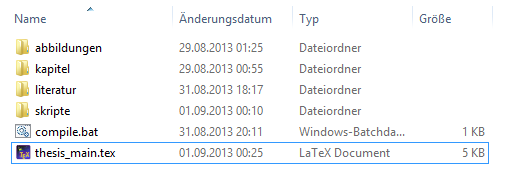
\includegraphics[width=1\textwidth]{verzeichnisStruktur}
        \captionsetup{width=1.0\textwidth}
        \capquelle{https://github.com/andygrunwald/FOM-LaTeX-Template}\label{figur-k1}
    \end{center}
\end{figure}

	\newpage
\section{Informationen vom Thesis-Day}
Siehe auch Wissenschaftliches Arbeiten~ \autocite[Vgl. ][Seite 1]{Balzert.2008}. Damit sollten alle wichtigen Informationen abgedeckt sein ;-)

\subsection{Pre-Anmeldephase}
\subsubsection{Vorüberlegungen}
Trichtermethode: Man beginnt mit der eigentlichen  Konklusion und überlegt dann, welche allgemeinen Teile dafür benötigt werden.

Welchen Mehrwert soll die Arbeit bieten \footnote{Diese Fußnote hat inhaltlich keinen Sinn. Es soll nur ein langer Text generiert werden, dass dieser Vermerk über zwei Zeilen reicht und bündig dargestellt wird.}? Auch darüber nachdenken, wie die Arbeit einen selbst weiter bringen kann. Studienverlauf prüfen. Welche Vorlesungen hat mich besonders interessiert? Wo liegen meine Stärken etc.

\begin{enumerate}
\item Themenfindung
\item Literaturrecherche
\item Gliederung/Motivationspapier erstellen
\item Betreuerauswahl (siehe Liste im \nomenclature{OC}{FOM Online Campus} OC)
\item Anmeldung (ab 141 Credits möglich)
\end{enumerate}

\subsubsection{Anregungen finden}
\begin{itemize}
\item \href{http://www.diplom.de}{www.diplom.de}
\item \href{http://www.hausarbeiten.de.de}{www.hausarbeiten.de}
\item Datenbanken aus Tools and Methods
\item etc.
\end{itemize}

\newpage
\subsection{Anfertigungsphase}
Die Anmeldung ist mittlerweile jeden Mittwoch möglich.

\begin{figure}[htbp]
    \begin{center}
        \raggedright\caption{FOM-Vorgaben zur Thesis im Online-Campus}
        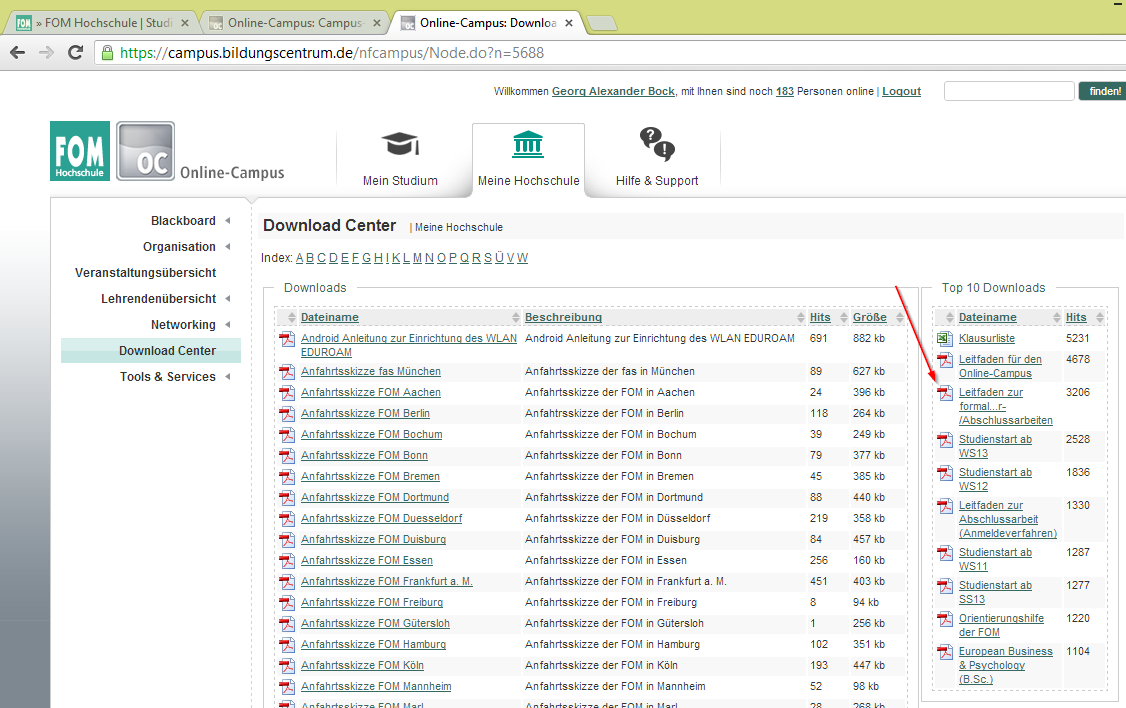
\includegraphics[width=1\textwidth]{campusDownload}
        \captionsetup{width=1.5\textwidth}
        \capquelle{https://github.com/andygrunwald/FOM-LaTeX-Template}\label{figur-k2}
    \end{center}
\end{figure}

Laut Herrn Keller sollte der Umfang der Thesis (für eine gute Note) eher im Bereich der 60 Seiten liegen. Wie immer ist das vermutlich mit dem Betreuer abzustimmen. Die Liste der Dozenten, die Abschlussarbeiten betreuen, findet sich auch im OC.

Zeit zur Erstellung der Thesis 2-4 Monate.

Es müssen zwei gedruckte Arbeiten abgegeben werden. Flüchtige Quellen als PDF ausgeben lassen und auf CD abgeben. Thesis zusätzlich digital einreichen. Beim Binden der Thesis auf Qualität achten. Haptik und erster Eindruck sind in der Bewertung \enquote{auch} wichtig. Arbeiten können in jedem FOM Studienzentrum abgegeben werden. 

\subsection{Post-Abgabephase}
Nach Abgabe ca. 2 Wochen bis zum Kolloquium.

Kolloquium:
\begin{itemize}
\item Dauer: 30 Minuten 
\item Präsentation (manche Prüfer wollen eine, andere nicht)
\item Betreuer vorher fragen was er möchte
\item Es gibt einen Frageteil, dieser bezieht sich auf die Arbeit, kann aber auch darüber hinaus gehen.
\item Der Tag des Kolloquiums steht auf der Endbenotung 
\item Thesis und Kolloquium sind zwei getrennte Prüfungsbereiche. Für beide gibt es nur zwei Versuche. 
\item Am Tag des Kolloquiums erhält man die Bestätigung, ob bestanden oder nicht
\end{itemize}

	\newpage

\section{Latex-Details}

\subsection{Verwendete Software, Editor und Zusatzpakete}
\subsubsection{Windows 8+}
\begin{itemize}
\item MikTex: 2.9, 32-bit
\item Biblatex: 3.5, Zusatz: Biber.exe
\item Editor: TexStudio (kann ich empfehlen), Notepad++
\end{itemize}

\subsubsection{Mac OSX und iOS}
\begin{itemize}
\item MacTeX: \url{https://tug.org/mactex}
\item Editor: TexPad \url{https://www.texpadapp.com}
\end{itemize}



\subsubsection{Online}
Overleaf ist eine Online-Anwendung mit der Ihr direkt im Browser an eurer Thesis schreiben könnt. Bis 1GB Größe und
maximal 60 Einzeldateien könnt ihr Overleaf kostenlos nutzen: \url{https://www.overleaf.com/}


\subsection{Dokumentenklasse}
Eigentlich hatte Prof. Finke empfohlen die Dokumentklassen \enquote{Book} oder \enquote{Report} für die Erstellung der
Bachelor-Thesis zu verwenden, da diese über weitere Gliederungsebenen verfügen. Ich verwende dennoch eine leicht
modifizierte Komaskript-Klasse \enquote{scrartcl}, mit der Erweiterung um eine Ebene. Siehe (skripte/weitereEbene.tex).
Das Skript stammt irgendwo aus den Netz und übersteigt meine \LaTeX{}-Fähigkeiten. Dadurch kann ich über eine weitere
Ebene in der Arbeit verfügen, ohne mich mit der Modifikation von Kapitel-Seiten rumschlagen~
\footcite[Vgl. ][Seite 5]{Tanenbaum.2003} zu müssen. Diese Quelle ist nur zur Demonstration und hat keinen inhaltlichen
Bezug hierzu. Es werden übrigens nur die Quellen im Literaturverzeichnis angezeigt, die auch referenziert sind.


\subsection{Grafiken}
Das Paket \textbackslash usepackage\{float\} ermöglicht es die Grafiken und Tabellen an der Stelle im Text zu
positionieren, wo diese im Quelltext stehen (Option H). Ansonsten würde \LaTeX{} diese dort unterbringen, wo es
typographisch sinnvoll wäre - das wollen wir ja nicht ;-).

Die Breite der Grafiken am Besten relativ zum Text angeben.

\subsection{Quellcode}
Quellcode kann auf unterschiedliche Arten eingebaut werden.
Zum einen kann es hier durch direktives Einbinden in der Kapitel-Datei geschehen.
\begin{lstlisting}
% Hier wird aufgezeigt, wie man eine Grafik einbindet, es wird also in der PDF angezeigt,
% da es in einem Quellcode-Listing steht.
% Auch wenn es hier faelschlicherweise als LaTeX-Befehl angezeigt wird.
%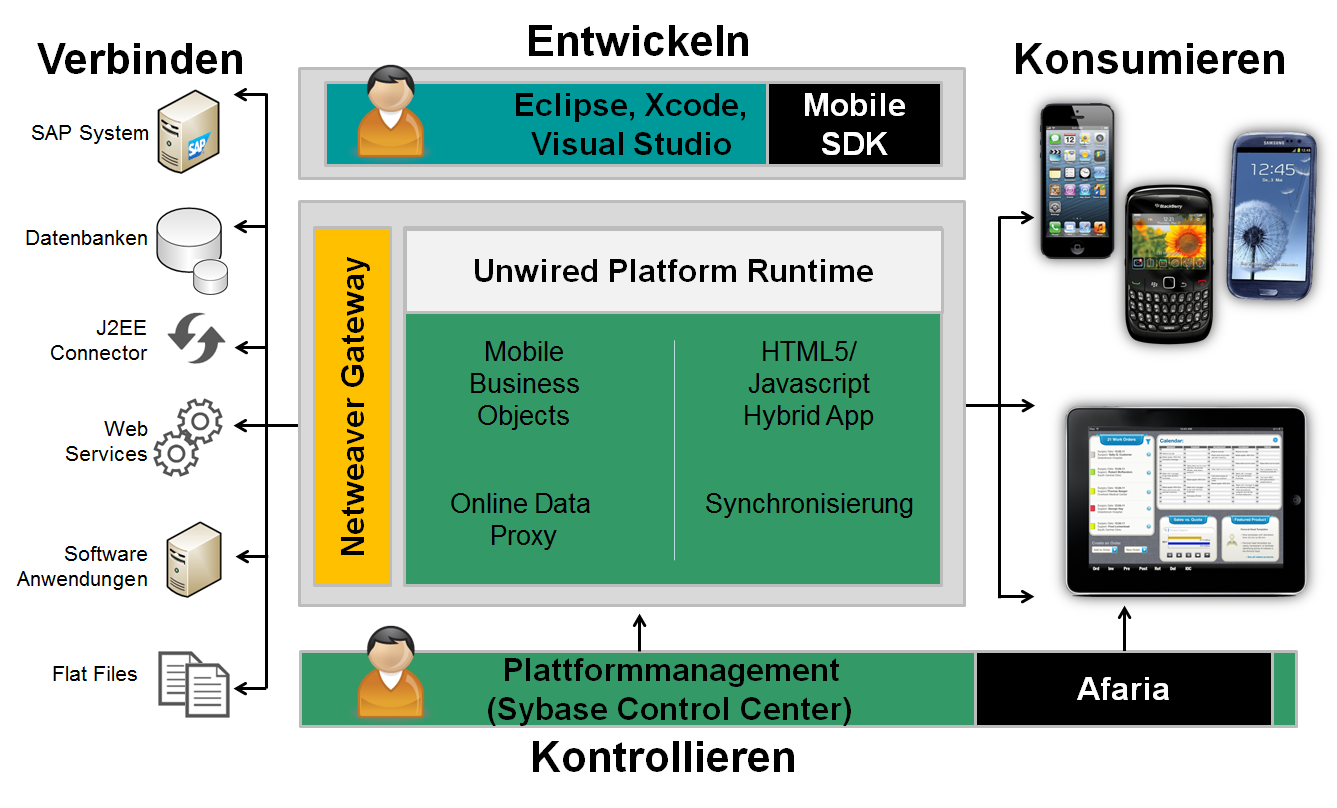
\includegraphics[width=0.9\textwidth]{sup}
\end{lstlisting}

Bei längeren Quellcode-Listings empfiehlt es sich jedoch auf eine externe Datei im Ordner Quellcode zu verlinken und diese einzubauen:
\lstinputlisting[language=HTML]{./Deine_Inhalte/Quellcode/Beispiel.html}

Da der Pfad zu den Abbildungen im Hauptdokument definiert wurde, muss hier nur noch der Name des Bildes ohne Dateiendung stehen (sup).

\begin{figure}[htbp]
	\begin{center}
		\raggedright\caption{Titel der Abbildung hier}
		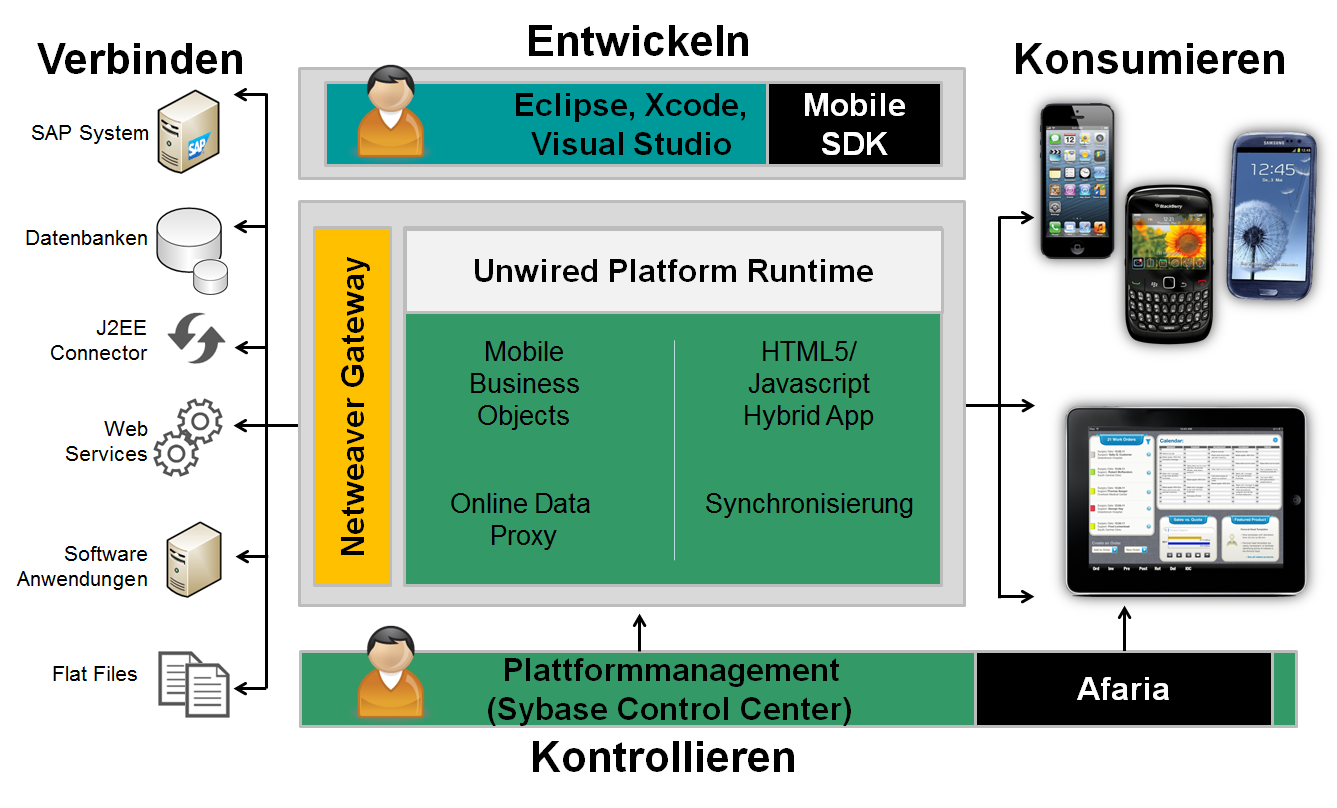
\includegraphics[width=1\textwidth]{sup}
		\captionsetup{width=1.5\textwidth}
		\capquelle{https://github.com/andygrunwald/FOM-LaTeX-Template}\label{figur-k2}
	\end{center}
\end{figure}

%\clearpage % hiermit werden alle Bilder Tabellen ausgeworfen

\subsection{Biblatex}
Von den vielen verfügbaren Literatur-Paketen habe ich mich für Biblatex entschieden. Die Anforderungen der
FOM\nomenclature{FOM}{Hochschule für Oekonomie \& Management} sollten hiermit erfüllt sein. Ich habe bisher nur Einträge
\enquote{@book} getestet. Wie immer steckt der Teufel hier im Detail und es wird sich später herausstellen, ob Biblatex
eine gute Wahl war. Die Anpassungen hierfür liegen unter skripte/modsBiblatex. Ich verwende das Backend Biber, welches
bib-Dateien in UTF-8 verarbeiten kann.

\subsection{Tabellen}
\begin{table}[H]
	\centering
	%\begin{tabular*}{\textwidth}{|l|l|l|}
	\begin{tabular}[ht]{|l|l|l|}
		\hline
		\textbf{Abkürzung} & \textbf{Beschreibung} & \textbf{Berechnung}\\
		\hline\hline
		MEK & Materialeinzelkosten & \\
		MGK & Materialgemeinkosten & $+ \uparrow$~*\\
		FEK & Fertigungseinzelkosten & \\
		FGK & Fertigungsgemeinkosten & $+ \uparrow$~*\\
		SEKF & Sondereinzelkosten der Fertigung & \\
		\hline\hline
		\multicolumn{3}{|l|}{\textbf{= Herstellungskosten}} \\
		\hline\hline
		VwGK & Verwaltungsgemeinkosten & $+ \uparrow$~*\\
		VtGK & Vertriebsgemeinkosten & $+ \uparrow$~*\\
		SEKVt & Sondereinzelkosten des Vertriebes & \\
		\hline\hline
		\multicolumn{3}{|l|}{\textbf{= Selbstkosten}} \\
		\hline\hline
		\multicolumn{3}{|l|}{+ Gewinnaufschlag} \\
		\multicolumn{3}{|l|}{+ Rabatte} \\
		\hline\hline
		\multicolumn{3}{|l|}{\textbf{= Nettoverkaufspreis (NVP)}} \\
		\hline
		\multicolumn{3}{|l|}{+ Umsatzsteuer} \\
		\hline\hline
		\multicolumn{3}{|l|}{\textbf{= Bruttoverkaufspreis (BVP)}} \\
		\hline
	\end{tabular} \\
	\caption{Beispieltabelle 1}
	\label{tbl:beispieltabelle2}
\end{table}

\subsection{Listen und Aufzählungen}
\subsubsection{Listen}
\begin{itemize}
\item ein wichtiger Punkt
\item noch ein wichtiger Punkt
\item und so weiter
\end{itemize}
\subsubsection{Aufzählungen}
\begin{enumerate}
\item Reihenfolge ist hier wichtig
\item Dieser Punkt kommt nach dem ersten
\item Da sollte jetzt eine 3 vorne stehen
\end{enumerate}

\paragraph{Tiefste Ebene 1}
Dies ist die tiefste Gliederungsebene. Sollten doch mehr Ebenen benötigt werden, muss eine andere Dokumentenklasse verwendet werden.

\paragraph{Tiefste Ebene 2}
Der zweite Punkt in dieser Ebene ist zur Erinnerung daran, dass es nie nie niemals nur einen Unterpunkt geben darf.
\footcite[Vgl. ]{website:andyGitHub:andysTemplate}


\subsection{Skript zum Kompilieren}
\subsubsection{Linux Unix Mac}
Latex will ja bekanntlich in einer bestimmten Reihenfolge aufgerufen werden:
\paragraph{Ohne arara Build Tool}
\begin{lstlisting}
#!/usr/bin/env bash
#Run the Script from the folder you are in...
CURRENT_DIR=$( cd "$( dirname "${BASH_SOURCE[0]}" )" && pwd )

pdflatex "$CURRENT_DIR/thesis_main.tex"
RETVAL="$?"
if [[ "${RETVAL}" -ne 0 ]] ; then
echo "First pdflatex run failed"
exit ${RETVAL}
fi

makeindex thesis_main.nlo -s nomencl.ist -o thesis_main.nls
RETVAL="$?"
if [[ "${RETVAL}" -ne 0 ]] ; then
echo "makeindex run failed"
exit ${RETVAL}
fi

biber "$CURRENT_DIR/thesis_main"
RETVAL="$?"
if [[ "${RETVAL}" -ne 0 ]] ; then
echo "biber run failed"
exit ${RETVAL}
fi

pdflatex "$CURRENT_DIR/thesis_main.tex"
RETVAL="$?"
if [[ "${RETVAL}" -ne 0 ]] ; then
echo "Second pdflatex run failed"
exit ${RETVAL}
fi

pdflatex "$CURRENT_DIR/thesis_main.tex"
RETVAL="$?"
if [[ "${RETVAL}" -ne 0 ]] ; then
echo "Third pdflatex run failed"
exit ${RETVAL}
fi

rm *.bbl > /dev/null
rm *.blg > /dev/null
rm *.aux > /dev/null
rm *.bcf > /dev/null
rm *.ilg > /dev/null
rm *.lof > /dev/null
rm *.log > /dev/null
rm *.nlo > /dev/null
rm *.nls* > /dev/null
rm *.out > /dev/null
rm *.toc > /dev/null
rm *.run.xml > /dev/null

echo "PDF Compile: Success"

exit 0
\end{lstlisting}
Dies ist der Inhalt des Skripts \enquote{Tools/compile.sh}.
\paragraph{Mit arara Build Tool}
\begin{lstlisting}
#!/usr/bin/env bash
#Run the Script from the folder you are in...
CURRENT_DIR=$( cd "$( dirname "${BASH_SOURCE[0]}" )" && pwd )

arara "$CURRENT_DIR/thesis_main.tex"
RETVAL="$?"
if [[ "${RETVAL}" -ne 0 ]] ; then
echo "arara run failed"
exit ${RETVAL}
fi

echo "Successfully compiled LaTeX PDF with arara"
exit 0
\end{lstlisting}
Dies ist der Inhalt des Skripts \enquote{compiletool.sh}.

\subsubsection{Windows}
Latex will ja bekanntlich in einer bestimmten Reihenfolge aufgerufen werden:
\begin{lstlisting}
pdflatex thesis_main.tex
makeindex thesis_main.nlo -s nomencl.ist -o thesis_main.nls
biber thesis_main
pdflatex thesis_main.tex
pdflatex thesis_main.tex
thesis_main.pdf
\end{lstlisting}
Dies ist der Inhalt der Batchdatei \enquote{Tools/compile.bat}.

	\section{Fazit}
Wünsche Euch allen viel Erfolg für das 7. Semester und bei der Erstellung der Thesis. Über Anregungen und Verbesserung
an dieser Vorlage würde ich mich sehr freuen.

Zu guter Letzt noch ein Fußotentest der im Fazit eigentlich nichts zu suchen hat.
\onlinecite{website:andyGitHub:andysTemplate}
\bookcite{jornal:addisonwesley:knuth}
\footcite[Vgl. ][Seite 5]{Tanenbaum.2003}
\fullfootcite{Beckert.2012}
\fullfootcite{Balzert.2008}
\fullfootcite{Tanenbaum.2003}
\textcite{Balzert.2008}


%====================================
% Literaturverzeichnis
%====================================
\newpage
\addcontentsline{toc}{section}{Literaturverzeichnis}
\pagenumbering{Roman} %Zähler wieder römisch ausgeben
\setcounter{page}{4}  %Zähler manuell hochsetzen

% Darstellung 1:
%\printbibliography %einfach alles

% Darstellung 2:
% Literaturverzeichnis nach Typ (@book, @arcticle, keine anderen Typen, gehe sicher das nichts fehlt!) sortiert.
% Dazu die Zeile (\printbibliography) auskommentieren und folgenden code verwenden:
%\printbibheading
%\printbibliography[type=article,heading=subbibliography,title={Artikel}]
%\printbibliography[type=book,heading=subbibliography,title={Bücher}]
%\printbibliography[type=online,heading=subbibliography,title={Webseiten}]

% Darstellung 3:
% Literaturverzeichnis nach Typ (@book, @arcticle (zusammen) und @online getrennt. Keine anderen Typen,
% gehe sicher das nichts fehlt!) sortiert.
% Dazu die Zeile (\printbibliography) auskommentieren und folgenden code verwenden:
%\printbibliography[type=book,heading=subbibliography,title={Literaturverechnis}]
%\printbibliography[type=article,heading=none]
%\printbibliography[type=online,heading=subbibliography,title={Internetquellen}]

	% Darstellung 4:
	\defbibfilter{noonline}{ \not{type=online} }
	\printbibliography[filter=noonline,heading=subbibliography,title={Literaturverzeichnis}] %alles anzeigen ausser '@online'
	\printbibliography[type=online,heading=subbibliography,title={Internetquellen}] %nur '@online' anzeigen

%====================================
% Eidesstattliche Erklärung
%====================================
	\newpage
\pagenumbering{gobble} % Keine Seitenzahlen mehr

%-----------------------------------
% Ehrenwörtliche Erklärung
%-----------------------------------
\section*{Eidesstattliche Erklärung}
Hiermit versichere ich, dass die vorliegende Arbeit von mir selbstständig und ohne unerlaubte Hilfe angefertigt worden ist, insbesondere dass ich alle Stellen, die wörtlich oder annähernd wörtlich aus Veröffentlichungen entnommen sind, durch Zitate als solche gekennzeichnet habe. Ich versichere auch, dass die von mir eingereichte schriftliche Version mit der digitalen Version übereinstimmt. Weiterhin erkläre ich, dass die Arbeit in gleicher oder ähnlicher Form noch keiner Prüfungsbehörde/Prüfungsstelle vorgelegen hat. Ich erkläre mich damit nicht einverstanden, dass die Arbeit der Öffentlichkeit zugänglich gemacht wird. Ich erkläre mich damit einverstanden, dass die Digitalversion dieser Arbeit zwecks Plagiatsprüfung auf die Server externer Anbieter hoch geladen werden darf. Die Plagiatsprüfung stellt keine Zurverfügungstellung für die Öffentlichkeit dar.

    \par\bigskip
    \par\bigskip
    \par\bigskip
    \par\bigskip

\begin{figure}[h]

    \begin{tabular}[h]{ll}
        \_\_\_\_\_\_\_\_\_\_\_\_\_\_\_\_\_\_\_ \hspace{1.5cm} & \_\_\_\_\_\_\_\_\_\_\_\_\_\_\_\_\_\_\_ \\
        Unterschrift & Ort, Datum \\
    \end{tabular}

\end{figure} %BiblaTex Deine_Inhalte/Literatur/litratur.bib
%====================================

\end{document}
